\documentclass[]{myTemplate}

\title{报告标题}
\author{作者}
\affil{下北泽大学}
\date{\today}

\newredbox{问题}{prob}
\newblackbox{注意}{notice}

\begin{document}
	\maketitle

	\begin{abstract}
		一段摘要正文。

		另一段摘要正文。
	\end{abstract}

	\section{某一节}\label{sec:1}
		实验仪器包括 WGD30 型光栅单色仪,汞灯,溴钨灯,三路输出电源,光电探测器(量程2\si{\volt}),
		样品(安装有0.5\si{\milli\metre}和1\si{\milli\metre}两种厚度的钕玻璃吸收片),显微镜(放大倍数20),
		聚光镜(焦距 $f = 60\si{\milli\metre}$,通光孔径$d = 30\si{\milli\metre}$)。

	\section{又一节}
	\subsection{一个小节}
		\begin{wrapfigure}{r}{0.32\textwidth}
			\centering
			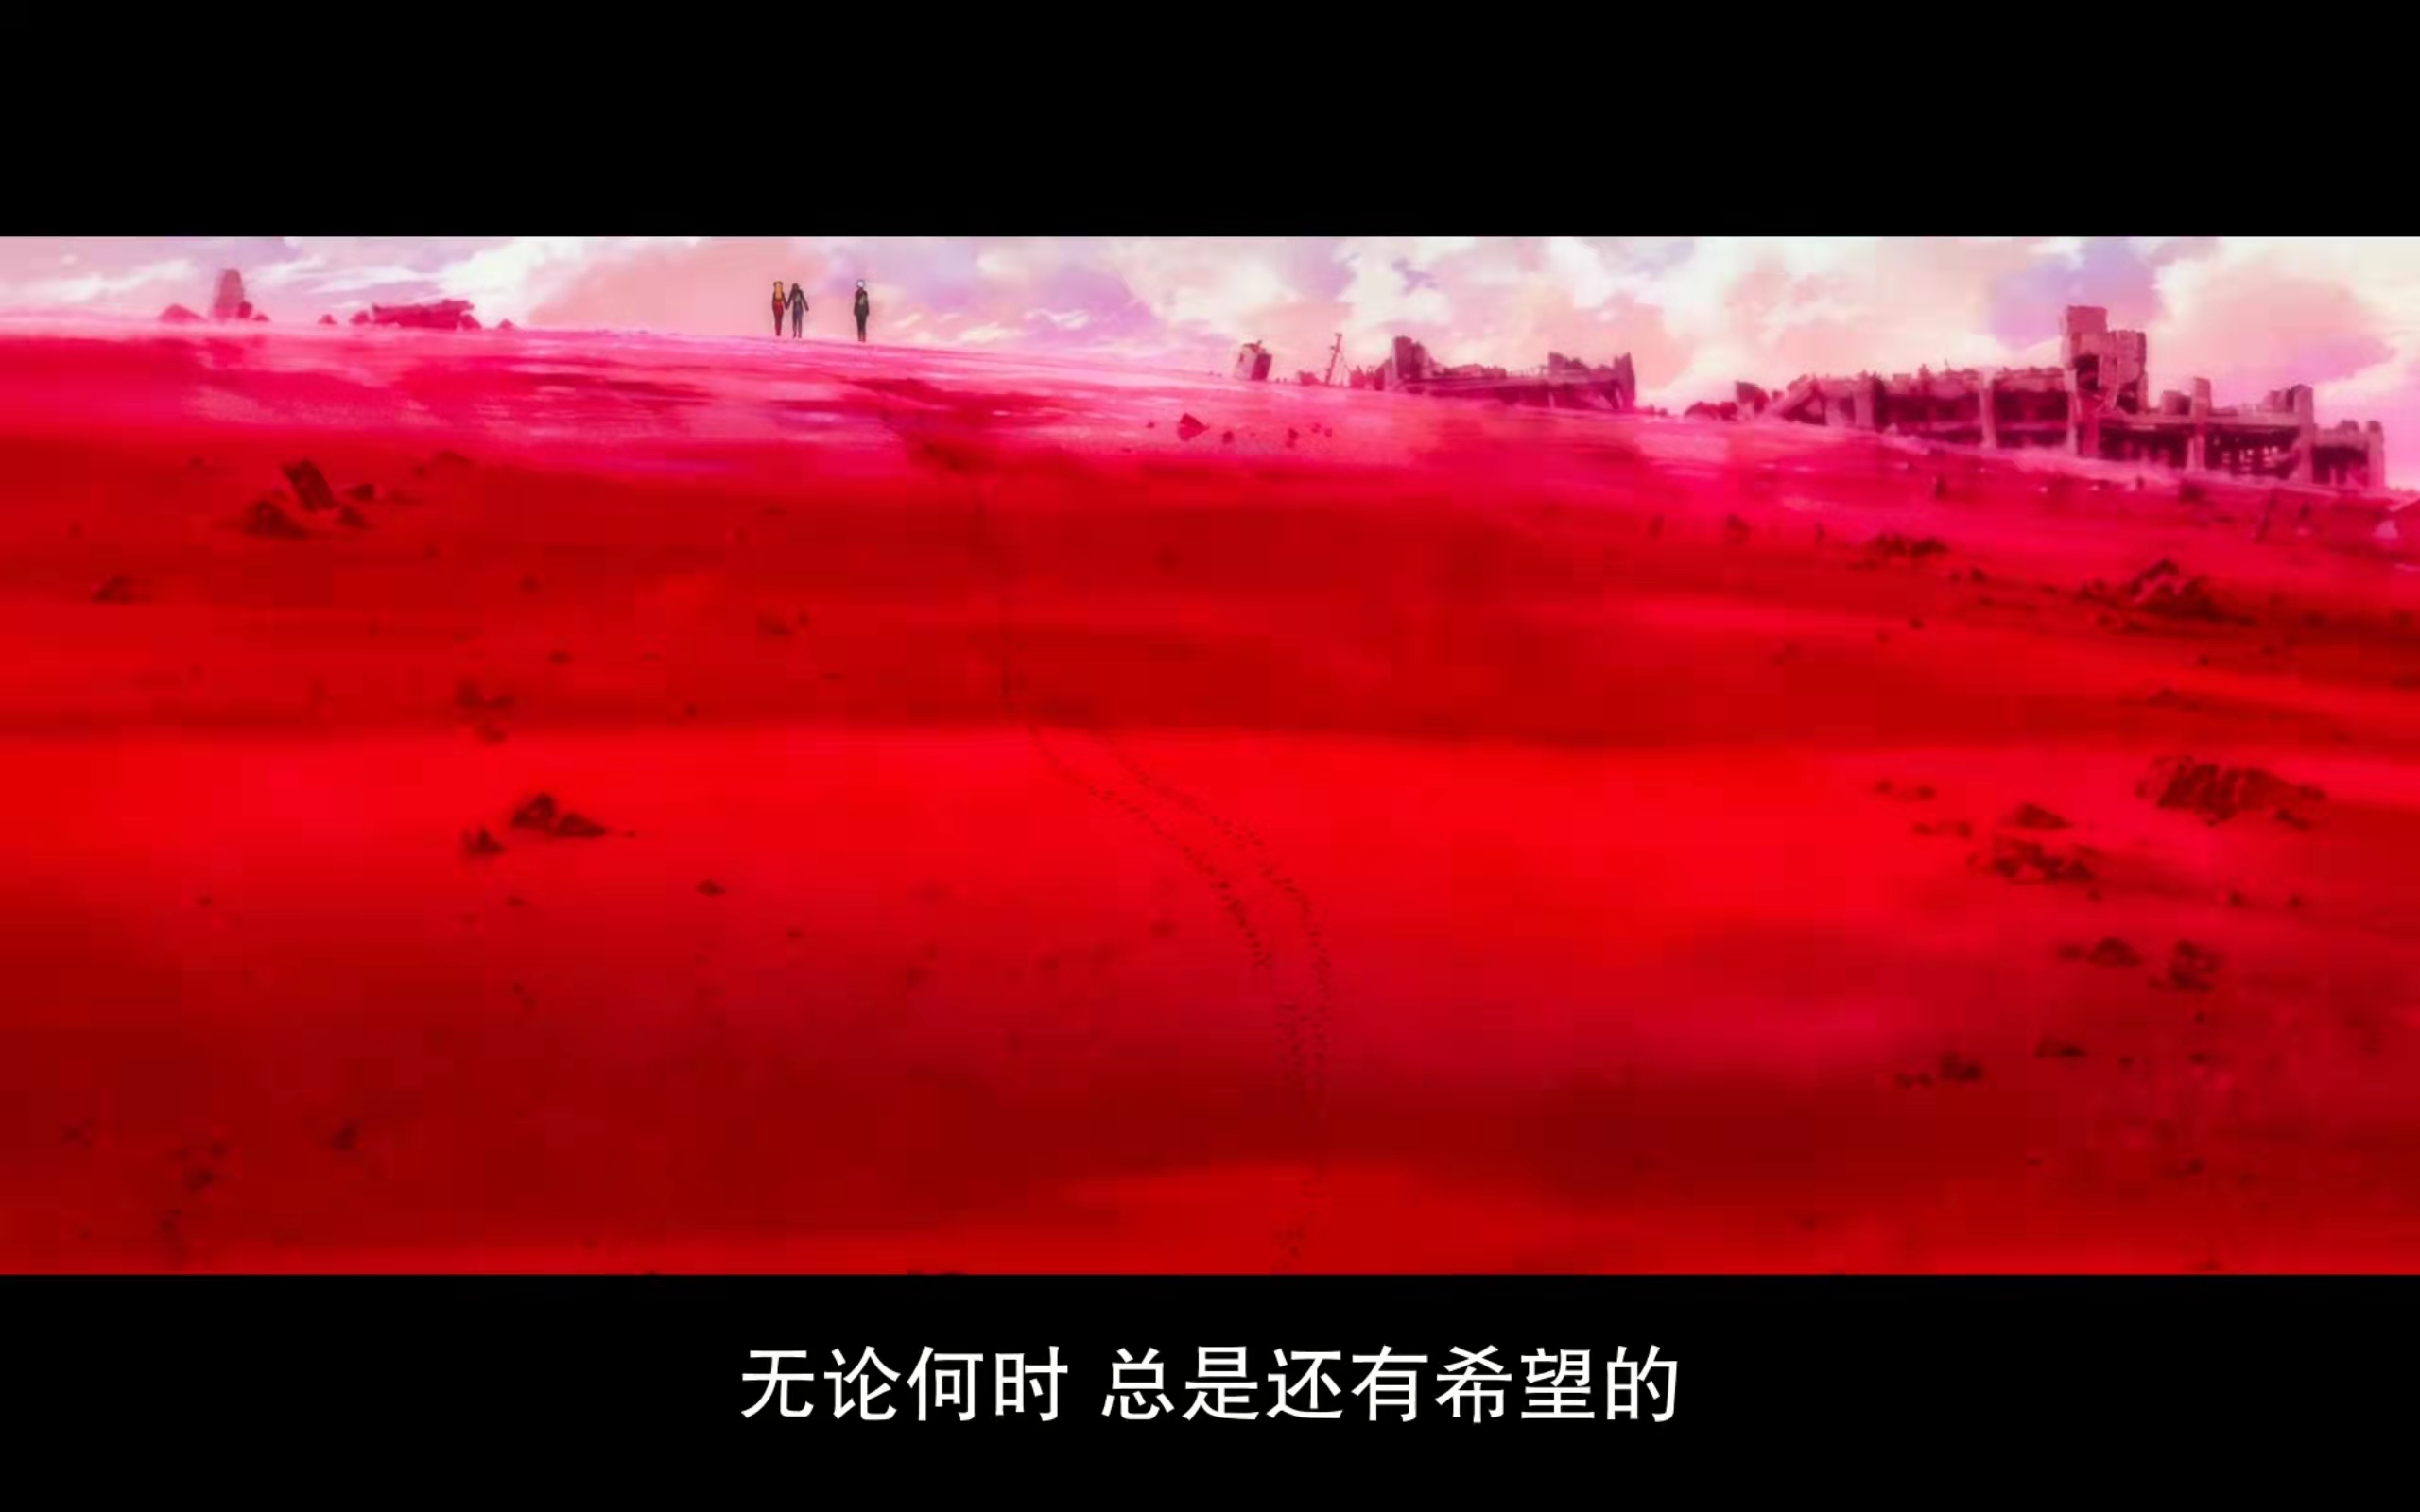
\includegraphics[width=0.32\textwidth]{sample.jpg}
			\caption{示例图片}\label{fig:1}
		\end{wrapfigure}

		此处为文字内容文字内容文字内容文字内容文字内容文字内容文字内容文字内容
		文字内容文字内容文字内容文字内容文字内容文字内容文字内容文字内容
		文字内容文字内容文字内容文字内容文字内容文字内容文字内容文字内容
		文字内容文字内容文字内容文字内容文字内容文字内容文字内容文字内容
		文字内容文字内容文字内容文字内容文字内容文字内容文字内容文字内容
		文字内容文字内容文字内容文字内容文字内容。

		以下为公式示例:
        
        $\Drivp{\bm{n}}{\xi^\alpha}=-b_{\alpha\beta}\bm{\rho}^\beta$,
		这是因为
		\begin{align*}
			&\drivp{\bm{n}}{\xi^\alpha}\cdot\bm{\rho}_\beta\\
			=&\drivp{}{\xi^\alpha}(\bm{n}\cdot\bm{\rho}_\beta) - \bm{n}\cdot\drivp{\bm{\rho}_\beta}{\xi^\alpha}\\
			=&-b_{\alpha\beta}
		\end{align*}
		
		\subsection{一个新的小节}
		此前,\cref{sec:1}中插入了\cref{fig:1}。

	\section{再一节}

		\begin{prob}[一种box示例]
			环境标题可在模板中修改。
		\end{prob}
		\begin{prob*}
            不带编号的相应box。
        \end{prob*}

		\begin{notice}[另一种box示例]
			此处为文字内容。
		\end{notice}

	\section{最后一节}
	代码块示例示例如\cref{lst:1}所示。
    \begin{lstlisting}[caption={sim.cc}, label=lst:1]

        #include "G4VUserDetectorConstruction.hh"
        #include "G4tgbVolumeMgr.hh"
        
        class DetectorConstruction : public G4VUserDetectorConstruction
        {
            public:
                G4VPhysicalVolume* Construct() {
                    G4tgbVolumeMgr::GetInstance()->AddTextFile("detector");
                    return G4tgbVolumeMgr::GetInstance()->ReadAndConstructDetector();
            }
        };
        //构造探测器,探测器描述在文件"detector"中
        
    \end{lstlisting}

\end{document}